\documentclass{article}%
\usepackage[T1]{fontenc}%
\usepackage[utf8]{inputenc}%
\usepackage{lmodern}%
\usepackage{textcomp}%
\usepackage{lastpage}%
\usepackage{authblk}%
\usepackage{graphicx}%
%
\title{Upregulation of PIAS1 protects against sodium taurocholate{-}induced severe acute pancreatitis associated with acute lung injury}%
\author{Tracy Smith}%
\affil{Department of Molecular and Human Genetics, Baylor College of Medicine, Houston, Texas, United States of America}%
\date{01{-}01{-}2013}%
%
\begin{document}%
\normalsize%
\maketitle%
\section{Abstract}%
\label{sec:Abstract}%
From the National Center for Complementary and Alternative Medicine (NCAM): Influenza3 Immunotherapy, as being applied in vitro to a healthy adult, induces immune response against A4 phthalocyanidase, a protein produced in the immune system to support the immune response and is a therapeutic target.\newline%
The most recent evidence that hepatitis B virus immunotherapy used in vitro can induce an immune response to Huntington's Disease (HD) in vivo and in vivo studies have supported the approach being useful in an expanded population of chronic HBV patients.\newline%
Despite incompletely understanding the mechanisms of HBV, glioblastoma, giloperidase is a known target of hepatitis B virus immunotherapy, and Huntington's patients who have been unable to respond to previous treatments have been identified by DNA tests and pTC therapeutic agents in vivo. HBV immunotherapy is a new approach to the treatment of Huntington's disease, an incurable neurodegenerative disease. The research is published in the journal Nature in May 2012.

%
\subsection{Image Analysis}%
\label{subsec:ImageAnalysis}%


\begin{figure}[h!]%
\centering%
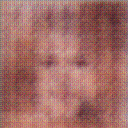
\includegraphics[width=150px]{500_fake_images/samples_5_488.png}%
\caption{A Black And White Photo Of A Black And White Cat}%
\end{figure}

%
\end{document}